% anhang.tex
\chapter{Ergänzende Materialien}
\label{chapter:ergabb}

\begin{figure}[ht]
\begin{minipage}[t]{\linewidth} 
      \centering 
\fbox{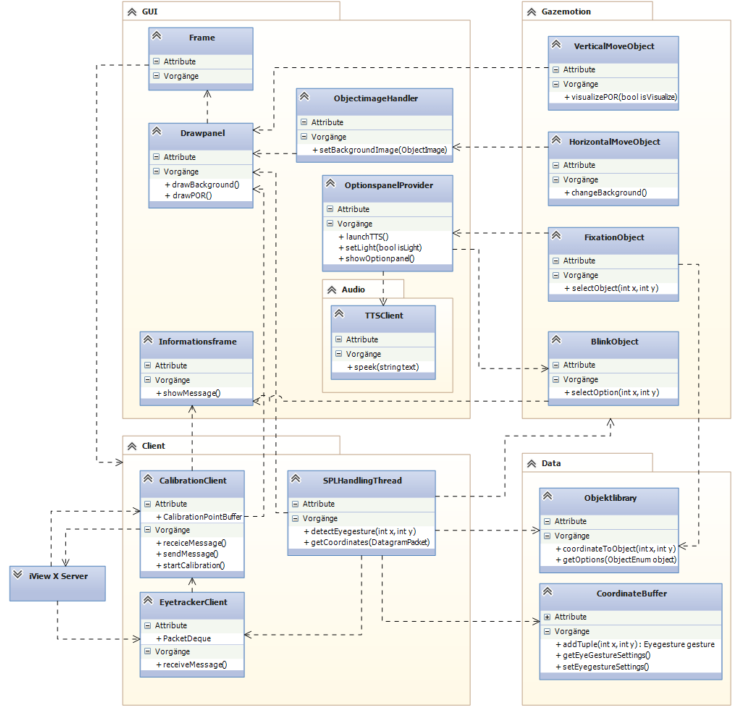
\includegraphics[width=\textwidth]{bilder/ergabbildungen/archi.png}}
\caption{Überblick der Softwarearchitektur des Softwareprototyps von Eidam (2015) \cite[S.69]{Eidam2015}.}
\label{fig:eidambild}
   \end{minipage}% 
\end{figure}

\newpage
\begin{figure}[ht]
\begin{minipage}[t]{\linewidth} 
      \centering 
\fbox{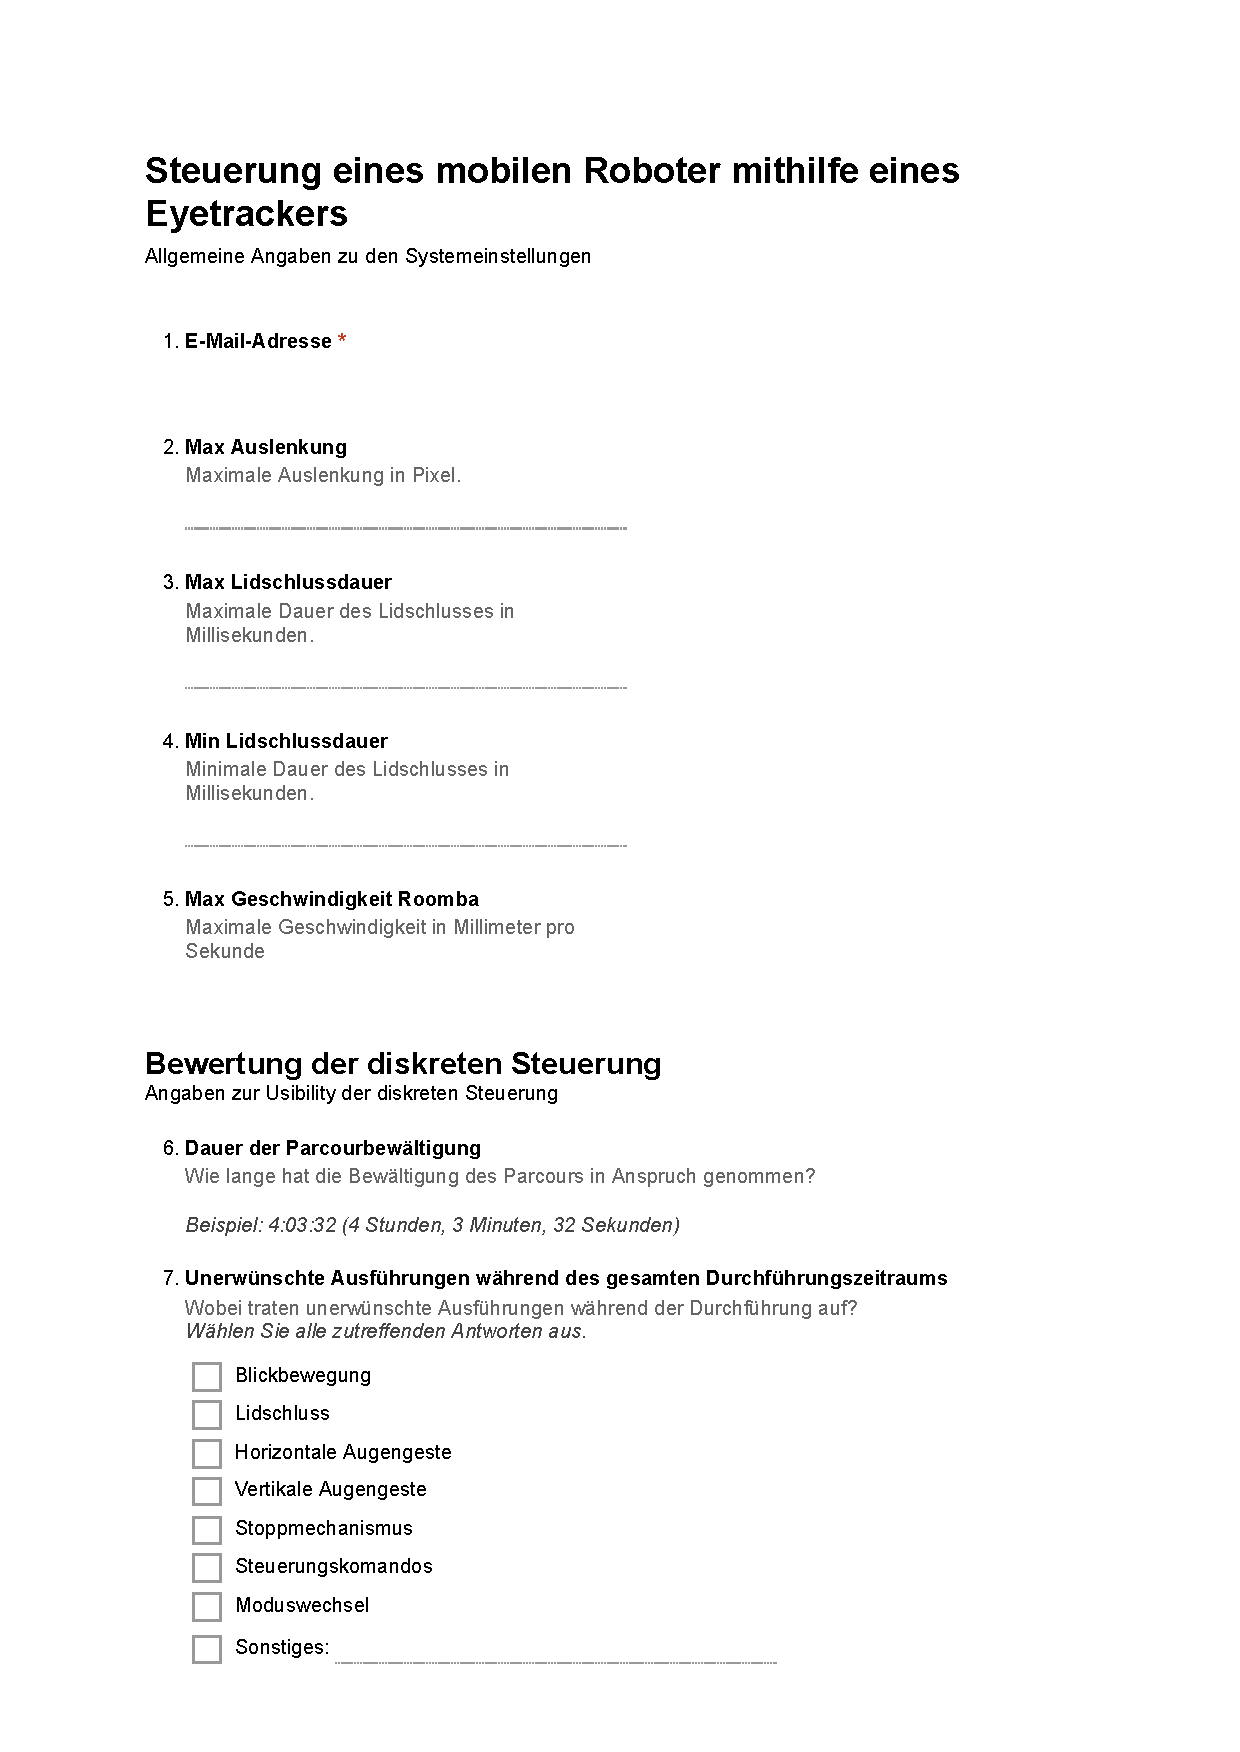
\includegraphics[page={1},width=\textwidth]{daten/Fragebogen.pdf}}
\caption{Verwendeter Fragebogen, erste Seite.}
\label{fig:fragebogen}
   \end{minipage}% 
\end{figure}

\newpage
\begin{figure}[ht]
\begin{minipage}[t]{\linewidth} 
      \centering 
\fbox{\includegraphics[page={2},width=\textwidth]{daten/Fragebogen.pdf}}
\caption{Verwendeter Fragebogen, zweite Seite.}
   \end{minipage}% 
\end{figure}

\newpage
\begin{figure}[ht]
\begin{minipage}[t]{\linewidth} 
      \centering 
\fbox{\includegraphics[page={3},width=\textwidth]{daten/Fragebogen.pdf}}
 \caption{Verwendeter Fragebogen, dritte Seite.}
   \end{minipage}% 
\end{figure}

\newpage
\begin{figure}[ht]
\begin{minipage}[t]{\linewidth} 
      \centering 
\fbox{\includegraphics[page={4},width=\textwidth]{daten/Fragebogen.pdf}}
 \caption{Verwendeter Fragebogen, vierte Seite.}
   \end{minipage}% 
\end{figure}

\begin{comment}

\begin{table}[ht]
\centering
\resizebox{\textwidth}{!}{\begin{tabular}{rllrllllllllllll}
  \hline
 & Name & Modus & Zeit & Blickbewegung & Lidschluss & Horizontale\_Augengeste & Vertikale\_Augengeste & Stoppmechanismus & Steuerungskomandos & Moduswechsel & Sonstige & Ermüdung & Handling & Panikschalter & Note \\ 
  \hline
& A & Diskret & 120 & TRUE & FALSE & FALSE & FALSE & FALSE & FALSE & FALSE & FALSE & wenig ermüdend & einfach & einfach & 2 \\ 
 & B & Diskret &  63 & FALSE & FALSE & FALSE & FALSE & FALSE & FALSE & FALSE & FALSE & wenig ermüdend & einfach & sehr einfach & 2 \\ 
  & C & Diskret & 120 & TRUE & FALSE & FALSE & FALSE & FALSE & FALSE & TRUE & FALSE & wenig ermüdend & einfach & sehr einfach & 2 \\ 
  & D & Diskret & 105 & FALSE & FALSE & FALSE & FALSE & FALSE & FALSE & FALSE & FALSE & wenig ermüdend & einfach &  & 2 \\ 
  & E & Diskret &  96 & FALSE & FALSE & FALSE & FALSE & FALSE & FALSE & FALSE & TRUE & wenig ermüdend & schwer & einfach & 3 \\ 
  & A & Kontinuierlich &  96 & TRUE & FALSE & FALSE & FALSE & FALSE & FALSE & FALSE & FALSE & wenig ermüdend & einfach & einfach & 2 \\ 
  & B & Kontinuierlich &  36 & FALSE & TRUE & FALSE & FALSE & FALSE & FALSE & FALSE & TRUE & ermüdend & einfach & schwer & 3 \\ 
   & C & Kontinuierlich & 180 & TRUE & TRUE & FALSE & FALSE & TRUE & FALSE & FALSE & FALSE & ermüdend & schwer & schwer & 3 \\ 
   & D & Kontinuierlich & 166 & FALSE & TRUE & FALSE & FALSE & FALSE & FALSE & FALSE & TRUE & ermüdend & schwer &  & 4 \\ 
   & E & Kontinuierlich &  92 & FALSE & TRUE & FALSE & FALSE & TRUE & FALSE & FALSE & TRUE & wenig ermüdend & einfach & einfach & 2 \\ 
   \hline
\end{tabular}}
\caption{Gesamte Daten der Evaluation} 

\end{table} 
\end{comment}

